\chapter{The Articulated Arm System}
\label{chap:AA}


\section{Description}

The Articulated Arm (AA) is a three-dimensional calibration device designed to deploy radioactive sources at specified points inside of the detector with an accuracy of one centimeter. The Articulated Arm consists of three principal parts: the stainless steel telescoping segments, which descend through the chimney into the target; the Lexan articulating segments, at the end of which are mounted the calibration source; and the motor assembly, housed in the glove box extension. A visual reference for these components can be seen in Fig. \ref{AA_Schem}. 

Scrupulous cleanliness standards were maintained, with metal elements of the AA which come into contact with target scintillator being electropolished before assembly in a room of ISO class 6, provided by Argonne National Lab. All other components of the AA which are expected to come into contact with the target scintillator have been cleaned before assembly with a hot Citronex solution in an ultrasonic bath, followed by hot nitrogen drying. The compatibility of the batches of material used in the AA with liquid scintillator have been examined by Double Chooz material compatibility experts and have been confirmed to not cause significant degradation of the scintillator after contact. This requirement is particularly important, given the challenges that the prior Chooz experiment experienced as a result of scintillator degradation. 

We will handle each subsystem in turn, beginning with the telescoping segments. After the primary systems have been addressed, the secondary subsystems for safety, control, and containment will be discussed. This will serve as an overview for the major components of the AA. 
 
\begin{figure}
\caption{Articulated Arm schematic, viewing the AA as if it were lying horizontally.}
\centering
\includegraphics[width=\textwidth]{AA/AA_Schematic.jpg}
\label{AA_Schem}
\end{figure}

\subsection{Telescoping Segments}
The telescoping segments consist of a set of 7 square, stainless steel (SS304) tubes that fit into each other as shown in Fig. \ref{Telescoping Segments}. The widest (top) section has a side dimension of 2.5 inches (63.5 cm) and each following section decreases in steps of 0.25 inches ((6.35 mm): 2.25 inches (57.15 mm), 2.00 inches (50.8 mm), 1.75 inches (44.45 mm), 1.5 inches (38.1 mm), 1.25 inches (31.75 mm) and 1 inches (25.4 mm). The wall thickness is 1/16 inch (1.59 mm). Sections are between 54.25 inches (1378 mm) and 53.5 inches (1359 mm) long. Fig. \ref{AA_Photo} shows a photograph of the retracted telescope lower part.

\begin{figure}
\includegraphics[width=.5 \textwidth]{AA/Telescoping_Segments.jpg}
\caption{Blueprint of the telescoping segments of the AA system from the side.}
\label{Telescoping Segments}
\end{figure}

\begin{figure}
\includegraphics[width=.5 \textwidth]{AA/AA_Photo.jpg}
\caption{Lower part of the telescoping segments. The system is in a retracted configuration.}
\label{AA_Photo}
\end{figure}

The telescoping system is designed to be compact when not deployed, but capable of reaching the bottom of the Neutrino Target of the far detector when fully extended. The tubes are guided through one another through a system of Delrin bearings, which fit into square holes at the bottom of each telescoping segment. Larger parts of the Delrin plates stick out inside the tube and keep the next section from falling through when the telescope extends. Details of the first section square tube and square holes are shown in Fig. \ref{Telescope bottom}. Details of the Delrin plates and the end cap on the top are shown in Fig. \ref{Delrin detail}. The Delrin bearings are also visible in white in the photograph of the telescope in Fig. \ref{AA_Photo}. 

\begin{figure}
\includegraphics[width=.5 \textwidth]{AA/Telescope_Bottom.jpg}
\caption{Detail of the bottom of the telescoping segments. Segments are upside down in this image.}
\label{Telescope bottom}
\end{figure}

\begin{figure}
\includegraphics[width=.5 \textwidth]{AA/Delrin_Detail.jpg}
\caption{Detail of the Delrin bearings from the front and side.}
\label{Delrin detail}
\end{figure}

The telescoping motion of the telescoping segments is accomplished through a series of black Delrin endcaps, which are attached to the top of each of the telescoping segments. The bottom segment has a coated stainless-steel cable (the $Z$-axis cable) attached to its endcap. When the $Z$-axis cable is pulled up, the bottom segment is pulled up until it contacts the endcap of the next segment, at which point continued pulling on the cable will cause the two to ascend in unison. Similarly, when the cable is lowered, the bottom segment and all segments with endcaps in contact with the endcap of the bottom segment are lowered. As the telescoping segments descend, the endcaps will catch, in order from top to bottom on the Delrin bearings of the next larger segment, causing the motion of that telescoping segment to stop, while the smaller segments are able to continue. Details of the endcaps can be seen in Fig. \ref{Endcaps}.

\begin{figure}
\includegraphics[width=.5 \textwidth]{AA/Endcaps.jpg}
\caption{Detail view of the endcaps both installed in a telescoping segment and by themselves. The dotted line indicates the path of the $Z$-axis cable running thought the center.} 
\label{Endcaps}
\end{figure}

\subsection{Articulating Segments}
The articulating segments are a series of round Lexan (polycarbonate) plastic segments of varying length with a diameter of 1.25". The chosen radial lengths bring the source at 350 mm, 650 mm, 850 mm, 1000 mm, 1050 mm and 1110 mm away from the $Z$-axis. These segments are attached to a stainless steel ``knuckle," which in turn is attached to the bottom of the smallest telescoping segment. Figure \ref{Knuckle_Attach} shows the details of the attachment of the articulating segments to the ``knuckle."

\begin{figure}
\includegraphics[width =.1 \textwidth]{AA/Knuckle_Attach.jpg}
\caption{The articulating segment (in green) screwed into the ``knuckle".}
\label{Knuckle_Attach}
\end{figure} 

The knuckle serves as the attachment point for the articulation cable, which allows the articulating segment to be articulating from a vertical orientation to a horizontal orientation. More detail about this function will be provided in Sec. \ref{sec: Motor Assembly}. 

At the end of the articulating segments is a source wand holder nut. There are two nuts used as part of deployment, one made of Lexan and the other of stainless steel. The source holder nut allows for the attachment of a radioactive source wand to the end of the articulating segment. The source wand slides into the source holder nut, after which the source holder nut is screwed on to the end of the articulating segments, locking the source wand in place. A picture of the final assembled articulating segment can be seen in Fig. \ref{Articulating Segment}. 

\begin{figure}
\includegraphics[width = .75 \textwidth]{AA/Articulating_Segment.jpg}
\caption{Articulating segment in the final configuration. In this image, the articulating segment is in the horizontal configuration.}
\label{Articulating Segment}
\end{figure}


\subsection{Drive Assembly}

\label{sec: Motor Assembly}
	The drive assembly contains many different components responsible for the motion of the AA system. A simplified overview of these systems can be seen in Fig. \ref{Drive_Assembly}.
	
	\begin{figure}
	\includegraphics[width = .5 \textwidth]{AA/Drive_Assembly_Edit.jpg}
	\caption{Simplified drive assembly in installed position. Does not include safety systems.}
	\label{Drive_Assembly}
	\end{figure}
	

	Motion of the AA is accomplished via two stepper motors, one in \emph{Z} and one in $\phi$, and a pneumatic piston, which controls the articulation and de-articulation of the articulating segments. The \emph{Z} stepper motor is connected to a drum, around which are wrapped two nylon-coated cables: one, the \emph{Z} cable, runs through the center of the telescoping segments and is attached to the top of the shortest of the telescoping segments, while the other, the articulation cable, runs over a pulley attached to the piston. After passing over the pulley, the cable runs down along the outside of the telescoping segments, and is attached to the articulating segments at the ``knuckle," the stainless steel interface between the telescoping and articulating segments. Motion in \emph{Z} is accomplished by turning the drum, which spools or unspools an equal amount of \emph{Z} and articulation cable. Accuracy within a given telescoping segment is better than one millimeter.
	
	The articulating segments are articulated through the use of a pneumatic piston, shown in Fig. \ref{Pully}. The piston moves a pulley, which retracts the articulation cable, pulling the knuckle up until the articulating segments are horizontal and contact the stop on the knuckle. The amount of pressure required to move the articulating segments into a horizontal position depends on the articulating segment used. Pressures range from 75 psi for the longest, 1050 mm segment configuration to 45 psi for the 350 mm configuration. If the pressure is too low, the system will not fully articulate, which can be confirmed by testing the tautness of the articulation cable in the glove box.  
	
	\begin{figure}
	\includegraphics[width =.5 \textwidth]{AA/Pully.jpg}
	\caption{The piston in the retracted (vertical) configuration.}
	\label{Pully}
	\end{figure}
	
	Pressure is delivered to the piston through a series of 1/4" hoses, which carry nitrogen from a cylinder located onsite. The hoses are routed through an electromagnetic solenoid, which can be switched to deliver the pressure to either part of the double-action piston, allowing for controlled motion for both articulation and de-articulation. Pressure from the piston is vented into the clean tent when the solenoid is switched. Speed of articulation and de-articulation is controlled by a flow-restricting valve on the line from the N$_2$ cylinder to the solenoid, as well as by flow-restricting valves on the outflow of the solenoid. 
		
	Motion in $\phi$ is controlled by a rotation table. The motion is smooth and accurate to within less than .01 degree, giving a position inaccuracy of much less than 1 mm. Use of the $\phi$-system, however, requires calibration of the motor before deployment in order to ensure smooth, continuous, predictable motion. This calibration can be performed when the AA is being installed in the Glove Box extension, before purging. No such calibration is required for the \emph{Z}-motor, but the arc of travel of the piston should be adjusted at this time as well, to ensure verticality and horizontality of the AA when articulated. 
	
	\subsection{Secondary Safety Systems}	
	The AA makes use of a number of safety systems, both in hardware and software, to ensure that there is no adverse effect on the capabilities of the far detector as a result of deployment. The motion of the AA is constrained to prevent unwanted contact between the AA and the walls of the target vessel. The constraints take the form of a trio of software limits: no motion below the center of the detector until articulation, no articulation until the AA is safely within the target, and no rotation within the range that is likely to cause contact between the AA and the filling tubes. These software limits are controlled through a Labview interface, which also provides for GUI-based control of the motion of the motors and the piston. The interface will be discussed in more detail in Sec. \ref{Software}.
	
	The software limits are backed by a pair of hardware limits, the home and forward switches, which act as ``kill switches" to prevent the AA from moving too far in \emph{Z}. The limit switches are attached to a side-plate on the AA, which features a large stainless steel screw to a brass plate.  As the drum turns to release cable, the screw turns at the same rate, moving the plate along the shaft. The plate contacts the whisker-triggered microswitches, which either stop motion, in the case of the home switch, or act as an ``Emergency Stop" in the case of the forward switch. The system can be seen in Fig. \ref{Whisker}. 
	
	In addition to the above limits, the \emph{Z} motor is subject to a torque limiter, to prevent over-tension in the cable in the event of a telescope failure. The torque limiter operates by limiting the voltage required by the motor for the $Z$-axis motion and therefore limiting the tension in the cable to prevent breaking. However, we were not able to stop the telescope from moving by holding it in place, suggesting that the torque limiter is not very sensitive. The lack of sensitivity implies that the telescoping segments would not stop immediately in case of AA getting stuck on the potential obstacle in the detector's chimney region. Therefore, special care has been taken to keep the AA centered and vertical in order to avoid any possibility of getting in contact with the chimney. 
	
	\begin{figure}
	\includegraphics[width =.5 \textwidth]{AA/Whisker.jpg}
	\caption{Home whisker switch in operational position.}
	\label{Whisker}
	\end{figure}
	
	In addition to the built-in hardware stops, the operator of the device has access to a manual emergency stop, which, when depressed, completely stops motion of the AA. In the event of a breach of the gas lines which operate the pneumatic piston, the flow of nitrogen can be stopped through the use of a quarter-turn valve, which is within easy reach of the operator. Furthermore, if there is a critical failure of all control systems, there is a manual retraction system which can be used to raise the AA into a completely retracted position without the use of software. 
	
	The retraction system allows for the $Z$-motor to be disengaged while the drive shaft is held in place with a pawl and ratchet system. The operator can then, making use of a ratchet stored within the glove box extension, slowly retract the telescoping segments without the risk of downwards motion. This system has been extensively bench-tested and validated. 
	
\subsection{Secondary Control System}
	\label{Software}
	Under normal operations, the AA operator will control the system entirely through the use of a Labview GUI. This interface not only controls the motion of the AA, but also keeps a history of commands which the AA has received, as well as regularly recording the position and status of the AA system. The Labview interface also provides feedback to the user on the position and status of the AA system both in numerical and graphical form. 
	
	
	 The Labview master interface relays commands to and receives information from the motors through two proprietary sub-programs. The first is Galil Tools, which controls the \emph{Z} motor and articulation solenoid. The second is Aerotech Soloist, which handles the $\phi$-motor. While the two programs are controlled through the Labview GUI in normal operation, they can be controlled independently in the event of a failure of one system or the other, as the GUI requires that both control systems are responsive for proper functioning. 
	 
	\subsection{Secondary Containment System}
	 When fully retracted, the entire AA is contained within a hermetically sealed containment system consisting of the Glove Box and Glove Box Extension. A cartoon of these systems, as well as the AA installed inside can be seen in Fig. \ref{GBE}. Tests have been performed to show the compatibility of the AA system with the glove box and its extension, as well as to validate that the systems can be purged and have well-constrained leak rates. These tests confirmed that the system does not trap oxygen, but instead is well-flushed with nitrogen when the Glove Box and Extension are purged in preparation for deployment. This procedure takes longer than the purging of the Glove Box alone, but can be accomplished within about a day of purging and maintained in a purged state overnight. Moreover, the total oxygen leak rate for the entire system was well under the safety limits established by the collaboration. 

\begin{figure}
\includegraphics[width = .5 \textwidth]{AA/GBE.jpg}
\caption{Cartoon of the AA system installed in the secondary containment system. View is from above and slightly to the left. Not all systems are included in the figure.}
\label{GBE}
\end{figure}

\section{Development and Testing}
Development of the AA system began early in the Double Chooz experiment. Initial designs for the AA used a rectangular cross section for the articulating segment, with almost all of the components of the AA being made of acrylic. Moreover, there was a movable collar that slides along the length of the articulating segment. A picture of this early design can be seen in Fig. \ref{Early Design}.

\begin{figure}
\caption{Early AA design, note the rectangular cross-section on the articulating segments and the sliding collar.}
\includegraphics[width=\textwidth]{AA/Early_Design.jpg}
\label{Early Design}
\end{figure}

In contrast, the final design is remarkably different. The articulating segments have a circular cross-section and are solid. The telescoping segments are 304 stainless steel, with the articulation cable being made of teflon coated steel. The point of attachment for the articulation cable has been moved closer to the central axis, and the sliding collar system (een in Fig. \ref{Collar}) has been removed, as it was not able to maintain a fixed position during motion of the telescoping segments. A picture of the modern design is in Fig. \ref{Recent_AA}.

\begin{figure}
\caption{Early AA collar design in detail.}
\includegraphics[width=\textwidth]{AA/Collar.jpg}
\label{Collar}
\end{figure}

\begin{figure}
\caption{Final AA design. The AA is being lifted by a crane, attached to the slings wrapped around the central telescoping.}
\includegraphics[width=.5 \textwidth]{AA/AA_Final.jpg}
\label{Recent_AA}
\end{figure}

The change from the early design to the modern design was a result of long term testing at Argonne National Lab. Rather than taking a chronological approach to the development, this section will be structured in an test-wise manner; that is, each test and its results will be discussed in turn. 


\subsection{Linearity Testing}
One of the more important questions about the motion of the AA is the nature of the motion produced by the stepper motors. Namely, is the motion linear with respect to the control system? If this is not so, is the non-linearity is well-understood? When a motion command is given, we must know the position in which the AA system will end up, in order to ensure safe, accurate calibration.  Linearity of motion was tested in two axes, the \emph{Z} motion axis and the $\phi$ motion axis. 

\subsubsection{\emph{Z} Motion Testing}
\emph{Z} motion accuracy testing was performed by mounting the system on a high platform, over 5 meters from the ground. The total length of the AA is 1.3 m longer than the distance available, allowing for all but the last telescoping segment to be extended. This test was performed by attaching a target (a small piece of white paper) to the tip of the source holder on the end of the articulating segment. The segment was not articulated during the test. A laser ranger was placed on the floor, and the beam of the laser ranger was pointed at a marked position on the target. The AA was then given a series of motion commands, and the distance from the floor to the target was measured with the laser ranger after each move. 
The internal position of the AA according to the software was recorded as well. The internal software position and the measured position from the laser ranger were then plotted against one another and a line was fit to the data. If the motion is linear and well-understood, the slope of the resulting line will be -1, as the ranger measures distance from the ranger to the target, which will decrease as the AA moves downwards, which is an increase in software position.

A graph of one of these tests can be seen in Fig. \ref{AA_Linearity}. The difference between the linear fit and the measured position is plotted in Fig. \ref{AA_Line_Residuals}. Both of these plots are in encoder counts, rather than other distance units, because encoder counts are the lowest level measurement that the software records. Each encoder count is one step on the $Z$-axis stepper motor.

\begin{figure}
\caption{AA linearity through laser ranger testing. Error bars are smaller than the size of the points.}
\includegraphics[width=\textwidth]{AA/Z_Vs_Counts_DOWN.jpg}
\label{AA_Linearity}
\end{figure}

\begin{figure}
\caption{Difference between the linear fit and the measured position in Fig. \ref{AA_Linearity}.}
\includegraphics[width=\textwidth]{AA/Residuals_Clean.jpg}
\label{AA_Line_Residuals}
\end{figure}

These early tests suggested a very linear relationship between physical \emph{Z} position and software-determined position. As a result, we are able to determine an accurate constant of proportionality between encoder counts, \emph{E}, and physical distance, such that we can speak in terms of software distance, \emph{S}, with $S= \alpha E$ where $\alpha$ is the calculated constant of proportionality. 

However, due to material compatibility requirements, the drum around which the cable was wound had to be changed from aluminum to stainless steel. The new drum had a smaller diameter than the previous drum, requiring a recalibration using the method described above.  During this change of the drum, the cables for the \emph{Z} motion and articulation were changed from an uncoated stainless steel cable to a teflon coated stainless steel cable. Because of the change of the cable, small non-linearities were introduced into the motion of the AA in \emph{Z}. 

Specifically, the weight of the telescoping segments causes a small stretching of the telescoping cable during motion. This has a very unusual effect on the \emph{Z} motion, as the teflon-coated telescoping cable supports the weight of the telescoping segments when the telescoping segments are not completely extended. When a segment is fully extended, however, the weight of the telescoping segment is instead supported by the other telescoping segments, as the now fully extended segment now rests on the white Delrin stoppers. 

Therefore, there is a step-wise non-linearity induced in the \emph{Z} motion of the AA. Whenever the AA undergoes a transition between moving segments, the weight of a segment is either added to or subtracted from the weight being supported by the teflon-coated $Z$-axis cable.  The change in the weight being supported causes a change of 2 mm in the physical \emph{Z} position of the bottom of the AA. Specifically, when the AA is moving downwards, the bottom of the smallest segment moves up by 2 mm per transition, as the weight is being taken off of the telescoping cable by the transition, while the situation is reversed when the AA is moving upwards. A graph of this behavior can be seen in Fig. \ref{Z-Non-Linearity}.

\begin{figure}
\caption{Weight-based \emph{Z} non-linearity in the AA system as a result of cable changes.}
\includegraphics[width=\textwidth]{AA/Transitions.jpg}
\label{Z-Non-Linearity}
\end{figure}

The \emph{X} axis of this graph is the position of the AA indicated by the control software. The \emph{Y} axis of the graph is the deviation from perfect 1:1 linearity. Error bars on the graph are from the error on the laser ranger, which has a listed error of $\pm$ 2 mm. 

In preparation for the deployment of the AA system, the AA was disassembled, electropolished, and reassembled in a clean environment. After reassembly, we tested the $Z$ linearity of the AA system again. These tests were conducted with the system mounted on a forklift, rather than with the system mounted in a high bay, as per the previous tests. This was due to the need to maintain material cleanliness between the clean assembly and the installation of the AA system in the Double Chooz Far Detector. One test was performed inside of the clean room where the AA was assembled, while the other took place in the physics support engineering bay at Argonne National Lab, with the system enclosed in a pair of plastic bags. 

These tests gave results consistent with those shown in Fig. \ref{Z-Non-Linearity}, although the short distance of the test only allowed for a single segment transition, which limited the validation power of the result. The position linearity was validated again onsite at the time of AA installation, under the same conditions (only one segment transition possible). A final confirmation of our model of the \emph{Z} motion of the AA will take place during deployment, where the position of the liquid level is well known, and it is possible to determine contact between the liquid and the AA system through the monitoring of the pressure of the Double Chooz liquids, which is sensitive to changes in pressure on the order of .01 milliBar. The ability of the pressure system to determine the position of the AA will be detailed in Sec. \ref{sec:Pressure Tests}.


\subsubsection{$\phi$ Motion Testing}
In addition to tests of the \emph{Z} motion linearity of the AA system, we performed tests to confirm the $\phi$ motion linearity in the summer of 2012. These tests took place at the engineering support bay of the HEP division of Argonne National lab. To perform these tests, we mounted the AA on a forklift and articulated the segments with a pressure of 90 psi applied to the articulation piston. We used the segment with total length of 100 cm,  and attached a laser ranger to the tip of the articulating AA. The laser ranger indicated a point on the ground directly below the position of the tip of the articulating segment, which we then marked. The AA was rotated by some amount, and the new position was then marked. We then measured the linear distance between adjacent pairs of marked points, which gave us three sides of a resulting triangle. One side being the measured distance between points being one side and the distance from the center of the AA system to the tip of the articulating segment being the other. We then calculated the angle opposite to the measured side, which should correspond to the angle rotated. The graph in Fig. \ref{Phi-Linearity} is the plot of measured rotation along the \emph{Y} axis against expected rotation along the \emph{X} axis. 

\begin{figure}
\caption{Measured angle compared to encoder-given angle with fit.}
\includegraphics[width=\textwidth]{AA/Phi_Linearity.jpg}
\label{Phi-Linearity}
\end{figure}

It is evident that the AA system has excellent linearity in $\phi$. Unlike with the \emph{Z}-axis system, there were no changes to the $\phi$-axis system during the course of development. However, to confirm the exactly linearity of the system, an additional test was performed in January of 2013, before the clean assembly of the AA. We used the same method detailed above. The results of this test were consistent with Fig. \ref{Phi-Linearity}. 

We did not perform an additional controlled test of the $\phi$ system after clean assembly, other than basic validation of motion and ``by eye" confirmation of proper function. This is because the coupling between the $\phi$-axis motor and the AA system is much simpler than the coupling between the AA and the \emph{Z}-axis system, as there are no intermediaries between motion of the motor and motion along the axis. Provided the motor remains calibrated (and re-calibration of the motor took place during installation), there is no possibility of a mechanical non-linearity being introduced. 



\subsection{Articulation Testing}
The AA system is lowered into the Neutrino Target with the articulating segments hanging vertically. Once the articulating segments are inside of the Neutrino Target, they are pulled into a horizontal position using the piston system described in Sec. \ref{sec: Motor Assembly}. The articulation positioning is much more complex than either of the other motion axes and, consequently, required a great deal of calibration and testing in order to get the movement to be accurate and well-controlled. 

The difficulties associated with this axis are three-fold. First, the segments are moved by way of a pneumatic piston, which naturally reduces control over the exact position of the axis to two possible states, articulated and de-articulated. Second, there is considerable variation in the length of the articulating segments, with the shortest measuring 350 mm from end to source wand tip, while the longest being 1050 mm in length. Finally, because the segments are being articulated in liquid scintillator, their motion is strongly affected by buoyancy and drag. Despite these challenges, we were able to calibrate and control motion along the articulation axis with error of less than a centimeter. 

\subsubsection{Droop Testing}
  The first thing that needed to be determined for the articulation system was the shape and structure of the articulating segments. A concern with the early design of the AA was droop, that is to say, deflection along the length of the AA because of the AA being supported only at the rear. This cantilevering not only is dangerous to the long term linearity of the AA, but also adds uncertainty to the vertical position of the AA. To measure the droop, we articulated the system and measured along the length of the articulating segment.  Originally, these tests were performed in air, but as the articulating part of the AA is supported by the force of buoyancy when it is deployed in the detector, these measurements are not good representations of the ``true" droop that the system will experience during deployment. Therefore, two additional sets of tests were conducted, one in water and one in oil. 
  
  Early tests showed a great deal of droop in the AA, as shown in Fig. \ref{Droop_1}.  Even worse, not only was the droop large, but it also varied with the configuration of the articulating segments. This is due to the early design of the articulating part of the AA, which consisted of a series of small segments which were screwed into each other. The connections between the segments acted as weak points which allowed for deflection. In a completely solid AA, the downward force varies with $R^2$, where \emph{R} is the length of the AA, resulting in a parabolic deflection. However, when weak points are introduced, as in the case of segments which are screwed into one another, each individual solid segment has its own parabolic deflection, which, in the case of solid segments submerged in water, is small. Additionally, the joint is deflected downwards by the weight of the subsequent segments, resulting in a different total deflection along the length of the AA depending on the ordering of segment sizes; having larger segments closer to the knuckle results in much less droop than having smaller segments closer to the knuckle.  
  
  \begin{figure}
  \caption{Early droop test showing \emph{Z} from the laser ranger along the 95 centimeter length of the AA articulating segment.}
  \includegraphics[width=\textwidth]{AA/Droop_1.jpg}
  \label{Droop_1}
  \end{figure}

To deal with the droop, the configuration of the articulating segments was changed from many smaller segments which are attached to one another to a single, larger segment of appropriate size. There is a balance to be struck in the determination of the size of the articulating segment. The larger the diameter of the articulating segment, the more pressure is required to articulate the segment, as the mass of the articulating segment is larger. However, a larger diameter provides more stiffness, which results in less droop. The mass of the articulating segment can be mitigated somewhat by using a segment with a hollow center, but this also reduces the stiffness of the articulating segment. 

We performed a series of calculations of the expected droop experienced by segments depending on diameter and wall thickness. A sample graph of these calculations can be seen in Fig. \ref{Calculated_Droop}. In this graph, some of the segments are calculated to have negative droop, which would indicate that the buoyant force is in excess of the weight. Such a configuration is a safety risk, as a segment which became unattached from the knuckle would strike the top of the target volume, causing cracking of the vessel. This risk is not acceptable, so positive buoyancy is not allowed for articulating segments. Moreover, such a system would not return to vertical in the absence of pressure on the piston, as we depend on the weight of the articulating segment to de-articulate the AA, rendering the system unable to travel through the 10 cm diameter chimney. We found that a solid segment of diameter 1 inch allowed for a deflection of 0.6 cm, and had a small net negative buoyancy, making it an ideal situation. 


\begin{figure}
\caption{Droop for solid or hollow articulating segments of varying wall thickness.}
\includegraphics[width=\textwidth]{AA/Calculated_Droop.jpg}
\label{Calculated_Droop}
\end{figure}


After this change, the droop of the AA was measured in water. This was accomplished by submerging the AA in a tank of water and articulating it. We then measured the distance from the top of the tank to marked points on the AA with a laser ranger. To ensure a clean measurement, the laser ranger was taped to a 1 meter long attachment (a photo of this set-up can be seen in Fig. \ref{Laser_Stick}), which was slid along the top of the tub. The top of the tub was validated as level through the use of a bubble level. A cartoon of this method can be seen in Fig. \ref{Droop_Water}.

\begin{figure}
\caption{Photograph of the laser ranger measurement setup. This photograph is from an early test in a shallow tub, but the experimental setup is the same for the deeper tub.}
\includegraphics[width= .5 \textwidth]{AA/Laser_Stick.jpg}
\label{Laser_Stick}
\end{figure}

\begin{figure}
\caption{Cartoon of the droop test technique used with the laser ranger.}
\includegraphics[width=\textwidth]{AA/Droop_Liquid_Test.jpg}
\label{Droop_Water}
\end{figure}

By comparing the positions given by the laser ranger, we determined the droop of the segment for a given configuration.  Since we are taking differences in distance, we have to take into account the effect of the index of refraction of water on the distances given by the laser ranger. The ranger works by firing a series of pulses with a known wavelength and using a combination of phase and time information from reflected pulses to determine distance. When the laser hits the surface of the water or oil, a portion of the pulse is reflected while the rest passes through the material. However, the wavelength of the light inside the liquid is not the same as the wavelength of the light in air, causing possible shifts in the phase information. This may not seem significant, but it does make a difference, as our tolerance for position error of the AA is 1 cm. Our tests, performed by comparing the known height of the tank to the laser-ranger-measured distance, indicated a total error of $\pm2$ mm.  

With these corrections, we compared the droop of two different segments in water: both 1 inch in diameter, but one was solid while the other had a 0.5 inch hollow cavity. Our data showed that the hollow segment exhibits excessive droop in comparison to the solid segment. A plot of one of these tests can be be seen in Fig. \ref{Solid_v_Hollow}.

The test confirmed our theoretical calculations qualitatively; however quantitatively, the way in which droop occurred was unexpected, with the segments being unaffected by droop for a distance before bending near the tip. A possible explanation for this behavior is uncertainty in the elastic modulus of the plastic, as values for similar polycarbonate plastics showed a great deal of variation.  

\begin{figure}
\caption{Solid and hollow articulating segments droop testing in water showing an unexpected droop profile for the hollow segment.}
\includegraphics[width=\textwidth]{AA/Solid_Hollow.jpg}
\label{Solid_v_Hollow}
\end{figure}

The goal of the water test was to get a rough determination of the amount of droop, as the buoyancy of water is approximately 25$\%$ greater than that of mineral oil. Therefore, use of this method will underestimate the true amount of droop. This over-compensation can be roughly corrected for by attaching a compact mass to the center of the articulating segment, the mass of which is equal to the ``missing" weight. By placing the mass at the center of the AA, we approximately compensate for the extra torque required in mineral oil/liquid scintillator. 

The compensation technique only works for the articulating segment, which has a uniform density, but not for the components on the tip of the articulating segment. To ensure that we had a complete understanding of the droop of the articulating segments, we performed the same test in mineral oil.  Mineral oil increases the error related to the laser ranger measurements of distance, but completely eliminates errors associated with buoyancy, as the density of mineral oil is very close to the density of the liquid scintillator in the target volume of Double Chooz. 

Despite these advantages, we experienced a number of problems with testing in mineral oil, primarily, the expense and the difficulty of containment. The tank we built to test the system in water was not usable with the mineral oil. We built a new tank as well as a secondary containment system to catch the small leaks of oil. To reduce possible sources of error in this final, oil-based measurement, we built new tank out of transparent plastic. This allowed us to measure the droop of the AA by pressing a pair of rulers against the transparent side walls, and observing the distance from the surface of the liquid surface to the articulating segment. Since the surface of the liquid will be exactly perpendicular to vertical, this gives a very powerful tool for determining droop.  A graph of the measured droop of one of the solid articulating segments in oil can be seen in Fig. \ref{Oil_Droop}.

\begin{figure}
\caption{Measured droop in oil with the ruler method (error bars inside points).}
\includegraphics[width=\textwidth]{AA/Oil_Droop_Ruler.jpg}
\label{Oil_Droop}
\end{figure}

As can be seen from Fig. \ref{Oil_Droop}, there is no real measurable droop in the AA system in oil to the level of precision of the ruler, $\pm$1 mm, which is an excellent situation. This is the same for all the articulating segments which were tested in the oil bath. With the conclusion of this test, we have an excellent understanding of the droop of the AA system. However, understanding the droop of the AA does not give a complete understanding of the motion of the AA when it articulates. To completely understand the motion of the AA, we needed to test and control the gas pressure in the pneumatic piston which causes articulation, as well as motion of the AA in the $X-Y$ plane when the AA articulates. 


\subsubsection{Pressure Testing}
\label{sec:Pressure Tests}
  The next challenge involved with the articulation system was determining the correct pressure setting to use. Originally, the goal was to have a single pressure for all configurations of articulating segments. This would allow for easier operation of the device, as well as more precise control, as most commercially available regulators are only accurate to $\pm$ 2 psi. However, early testing revealed that the range of pressure under which successful operation can take place is  small. Too little pressure causes the AA to ``hang" at certain points, and not fully articulate, while too much pressure at articulation causes motion in the $X-Y$ plane, and, at very high pressures, can cause the AA to de-telescope by roughly 1 centimeter.  We therefore needed to determine an articulation pressure for each articulating segment.
  
Testing the pressure required for articulation was done alongside with testing the droop of the AA system. This is due to the need for a liquid medium to ensure that the articulation pressures used in the tests are an accurate reflection of the articulation pressures needed for the AA inside the detector. Despite the small range over which proper articulation is possible, determining if the AA is completely articulated is straightforward, as the AA cannot articulate beyond 90 degrees, due to a hard stop on the knuckle. Moreover, when the pressure is insufficient to completely move the system to the horizontal configuration the point of stoppage is generally at about 30 degrees, well short of the 90 degrees required and easy to notice.

As part of the test, we validated that the AA was completely articulated by measuring the slope of the articulated segment after articulation. Since the droop is best modeled by a quadratic, we can disentangle the effects of droop from the effects of incomplete articulation. Moreover, since the measured droop in the final configuration is negligible, errors from mistaking droop for non-horizontality are minimal. 

Through testing, we developed a specific gas pressure required in the pneumatic piston for optimal articulation of each articulating segment. These values range from 45 PSI  (for the 350 mm segment) to 75 PSI (for the 1050 mm segment). These values allow for complete, repeatable articulation. 

\subsection{Planar Motion}
  A major concern involved with the articulation of the AA is in-plane motion. That is, when motion occurs in the plane of the detector (as opposed to along the \emph{Z} axis) either as the result of normal \emph{Z} motion with an AA which is not perfectly leveled or as a result of articulation. In either case, the in-plane motion restricts the lengths of AAs that can be used by the system, as in-plane motion threatens to cause parts of the AA (either the telescope or the articulating segments) to come into contact with the target vessel, potentially causing a breach of the vessel. 
  
  In order to avoid a breach of the vessel, we must restrict the choices of articulating segments such that the total length of the AA plus the in-plane motion gives a solid margin of safety (10 cm) around the edge of the veto. Both parts of the motion must be characterized in order to determine the articulating segments used during deployment. To do this, we need to see the effect of telescoping on motion in the \emph{X-Y} direction, motion which is primarily caused by improperly leveling the system, as well as the motion that is induced by articulation.
  
  
  \subsubsection{Telescoping Planar Motion}
  When the AA was designed, the question of leveling was assumed to be resolved by the tolerances between the telescoping segments. More accurately, the telescoping segments are basically hanging from the \emph{Z}-motion cable, and therefore, will tend to plumb themselves. Furthermore, since the fit between the telescoping segments has some space (1-2 mm), there was an assumption that small amounts of mis-leveling would not cause a problem. During testing, there was a critical failure caused by telescoping segments not descending in the proper order, which was determined to be caused by mis-leveling and too snug of a fit between the Delrin bearings and the telescoping segments. Though this potential failure mode has been prevented through the use of the torque limiter, there were other considerations. When we took a detailed scan of distance between the laser ranger and a point on the telescoping segments as a function of the \emph{Z} position of the bottom of the AA, we found a strong relationship between segment transitions and the measured position of the telescoping segments, indicating that a great deal of compensation for off-verticality is taking place, as can be seen in Fig. \ref{Telescoping_Planar}.
  
  \begin{figure}
  \includegraphics[width=\textwidth]{AA/Z_Motion_11_11.jpg}
  \caption{Measured planar positions of the telescoping segments as a function of \emph{Z} motion.}
  \label{Telescoping_Planar}
  \end{figure}
  
 These results were with an unleveled AA system. When the AA is properly leveled, these problems disappear. Specifically, we found that if the AA can be leveled to within 2 degrees, there is no measurable planar deviation at the bottom. Moreover, when installed in the glove box, there are many points at which the AA can be leveled to well within two degrees, allowing the effect of planar motion caused by the telescoping motion of the AA to be ignored.  
  
  \subsubsection{Articulating Planar Motion}
  While the planar motion caused by the telescoping of the AA system can be reduced to negligibility, that is not so for the in-plane motion caused by articulation. In order for the AA to correct non-verticality during decent, the telescoping segments are not a perfectly tight fit with one another. As the point of attachment of the articulation cable is slightly offset from the center-line of the telescoping segments, when the cable is pulled upwards there is a natural swing of the telescope in the direction of the pull. This swing is small, and the AA does tend to return back to its initial position in-plane, but must be accounted for when determining the articulating segments to use. 
  
  We tested the motion caused by articulation during our pressure and droop testing in mineral oil. We found that the motion of the AA varies strongly with not only the pressure used for articulation, but also with the flow rate of the gas. The speed of the gas controls the speed of the piston motion and consequently speed of articulation. A slower speed of articulation results in smaller amount of forward planar motion. While this result is unsurprising, it necessitates the use of a needle valve as part of the AA gas system to ensure a constant flow rate of the gas provided to the piston, such that the motion caused by articulation is repeatable. 
  
  With the installation of the needle valve, we were able to repeatedly articulate the system and measure the in-plane motion. We found that with the speed and pressure properly regulated, motion in plane was between 2 and 4 millimeters in the direction of articulation, and surprisingly, 2 millimeters of motion in the direction perpendicular to articulation. These results varied from articulating segment to segment, but were consistent for a given articulating segment. Motion in the perpendicular direction was not expected, and when investigated, turned out to be due to the loose fit of the articulating segment in the knuckle. The articulating segment is attached to the knuckle with a single pin, and therefore, is free to slide back and forth (in the perpendicular direction) within the interior of the knuckle during articulation, approximately 2-3 mm. Thus, when the AA articulates, there is a resistance to the motion from the liquid viscosity, resulting in currents which act on the articulating portion of the AA with sufficient force to cause the telescope to shift in the perpendicular direction. While the perpendicular motion is less of a concern to the safety of the detector than the motion in the direction of articulation, it still must be taken into account when data from the AA is analyzed. 
  
  In addition to the measured motion, we found that there is a non-trivial offset of approximately 2 millimeters in the direction of motion. This offset is small but repeatable and must be taken into account during analysis, as shifts on the millimeter level are detectable in the neutron capture efficiency, as shown in work by Julia Haser \cite{Julia_Efficiency}. There is no displacement in the perpendicular direction, which matches our understanding of the motion induced in the perpendicular direction. 
  

\subsection{Liquid Pressure Validation}
 A concern with the deployment of the AA was liquid displacement. Even though the larger telescoping sections of the AA are hollow, the total volume displaced is about 3 liters.  Should the amount of liquid being displaced be too large, the excess pressure produced on the liquid could cause the walls of the chimney to break. To prevent problems a breakage of the chimney due to natural pressure variation, the Double Chooz detector has an XTOS system designed to remove displaced liquid scintillator to a secondary containment system.  
 
 Unfortunately, the XTOS system is very slow to respond, necessitating a slow motion of the AA while inside of the liquid. To test how quickly we could move the AA system in the \emph{Z} direction while immersed in the target scintillator, we conducted displacement tests. These tests involved a quantity of mineral oil in a large cylinder of 12 cm in diameter. Since the chimney is 10 cm in diameter, adjustments had to be made to compare the results of the tests to the displacement that would result from a true deployment \cite{Archimedes}. 


We lowered the AA system into the liquid and measured the amount of liquid displaced as a result. A graph of the amount displaced as a function of the amount of AA submerged can be seen in Fig. \ref{Submerged}. It is clearly visible that the articulating segment used makes a large difference in the total amount of scintillator displaced. This is because the articulating segments, as mentioned before, are solid, while the telescoping segments are hollow. Thus, when the articulating segments are entering or leaving the liquid is the moment of greatest concern over an overpressure caused by liquid displacement. This is confirmed in the instantaneous (as opposed to total) liquid displacement plots in Fig. \ref{Delta_Submerged}. 

\begin{figure}
\includegraphics[width=\textwidth]{AA/Total_Displacement.jpg}
\caption{Total amount of liquid displaced as a function of \emph{Z} position and articulating segment.}
\label{Submerged}
\end{figure}


\begin{figure}
\includegraphics[width=\textwidth]{AA/Differential_Displacement.jpg}
\caption{Amount of liquid displaced per centimeter of motion in \emph{Z} as a function of \emph{Z} position and articulating segment. The steep rise in each graph corresponds to the immersion of the solid articulating segment, while the flatter portion of the graph corresponds to the hollow telescoping segments entering the liquid.}
\label{Delta_Submerged}
\end{figure}


These tests indicated that the AA must be moved very slowly when entering or leaving the liquid. However, moving at a speed of 1 -- 5 \hbox{\rm mm/s} will allow the AA to enter the liquid without resulting in an overpressure at the bottom of the target vessel. 



\label{Articulation Tests}

\section{Simulation}
	Further validation and justification of the AA was performed by simulating device performance in GEANT4 \cite{G4}. These simulations were designed both to provide a benchmark for comparisons once the device is deployed. Simulations were handled within the DCGLG4-sim framework \cite{DCGLG4sim}. Pictures of the AA system implemented in the DCGLG4-sim framework can be seen in Fig. \ref{DCGLG4}. 
	
\begin{figure}
\caption{AA implementation in DCGLG4sim showing relative positioning.}
\includegraphics[width=\textwidth]{AA/4_13_Cal_Group_Pres_01.jpg}
\label{DCGLG4}
\end{figure}


\subsection{AA Reconstruction Accuracy}

The first test that was performed in simulation was the validation of the ability of the DC position reconstruction software to determine the location of the AA-deployed source. This is a major concern, as the AA system depends entirely on dead-reckoning for position determination in \emph{Z} and $\phi$. In the event that the articulation of the AA is not complete, the ability of an operator to visually distinguish between a system which is fully articulated and a system which is merely almost completely articulated is low. Therefore, it is vital to be able to know to what the accuracy of the ``built in" position reconstruction system of Double Chooz is, to determine if it can be used to cross-check the position of the AA source.

There are two parts to this test. The first is the accuracy of the reconstruction software, while the second is the speed at which data from the detector can be processed and made available to the operators. The answer to the first question is the one that will be addressed in this section, while the second question will be answered in the Sec. \ref{sec:Deployment}.  We begin to answer the first question by ``deploying"  a source at various points in the detector and examining the reconstruction that is produced as a result. 

The simulations made use of a mono-energetic neutron source of 2 MeV. The points were generated at a single location, reflecting the point-like nature of the source inside the detector, and were smeared out by neutron thermalization and the reconstruction process. The distribution of reconstructed positions in the simulation was well described by a 3-dimensional Gaussian, as can be seen in the plot in Fig. \ref{Sim Reco}.

\begin{figure}
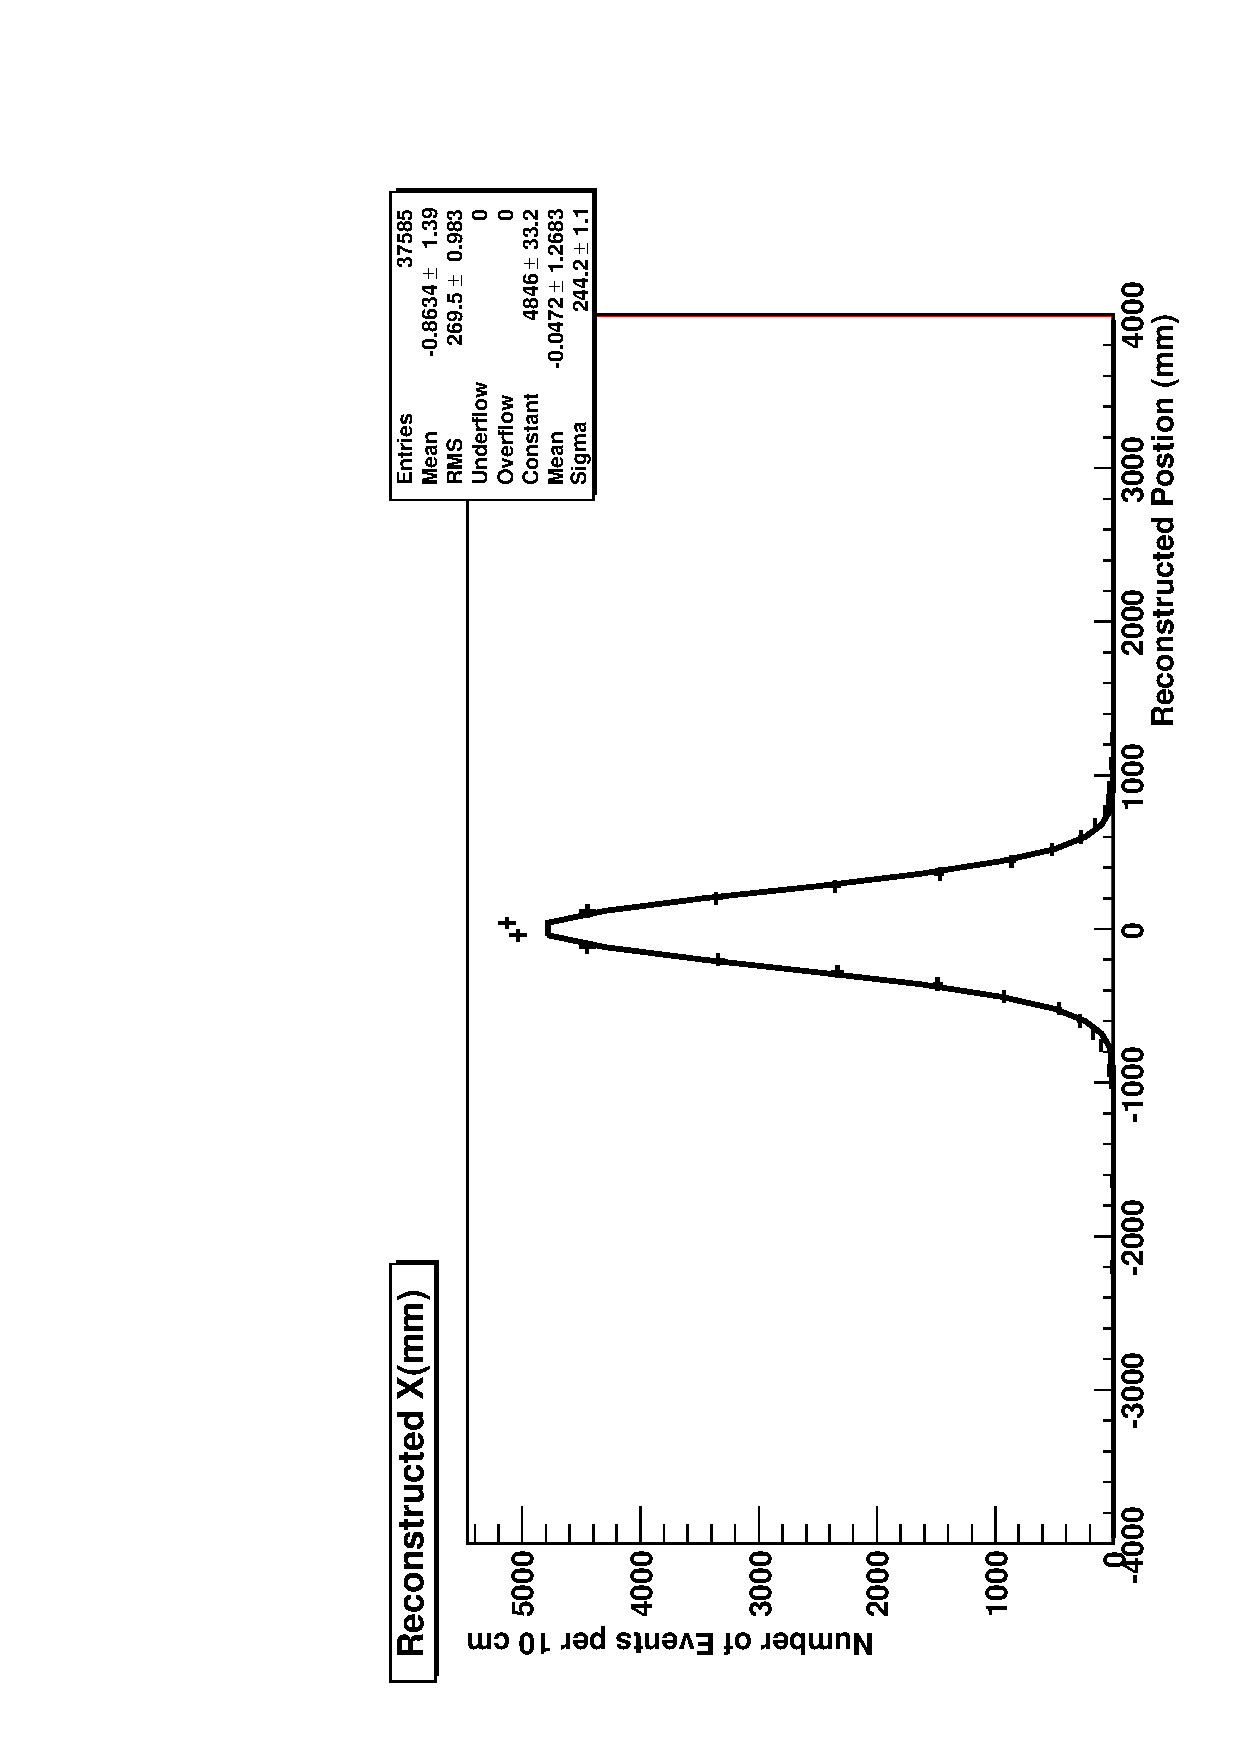
\includegraphics[width=\textwidth]{AA/AA_Reconstructed_Positions.jpg}
\caption{Distribution of reconstructed positions in DCGLG4sim showing rough Gaussianity in one dimension.}
\label{Sim Reco}
\end{figure}

Since the reconstructed signal is roughly Gaussian, we can model our ability to validate our position as our ability to distinguish between two nearby Gaussians. If we want a 3$\sigma$ confidence in the position at which the source is deployed, we need to be able to distinguish a source deployed at position \emph{X} with a source deployed at position \emph{X} + $\Delta$ more than 99.7\% of the time. The subsequent mathematics will be performed in 1-D, as that simplifies calculations, but can be expanded to 3-D without complication. 

The probability that an event generated by a source deployed at position \emph{X} will be reconstructed at position $\theta$ is given by the equation $P(\theta | X) =\frac{1}{\sqrt{2 \pi \sigma^2}}e^{\frac{-(\theta - X)^2}{2 \sigma^2}}$ . If you assume that the source does not move ($\Delta =0$) then the probability distribution of the reconstructed distance between two events, \emph{d} is given by $P(d | X, \theta) = P(\theta_1 - \Theta_2 | X, \Theta)$. Thus $P(d | X, \theta) = \frac{1}{\sqrt{4 \pi \sigma^2}}e^{- \frac{d^2}{4 \pi \sigma^2}}$ . Assuming we require a margin of confidence $\alpha$, we reject a ``motion" of the source if: $\int_d^{\infty} P(\rho) \delta \rho <1- \alpha$. In other words, we reject if $Erf(\frac{|d_i|}{2*\sigma} )> 1- \alpha \rightarrow P(reject | \Delta, \sigma) = .5 \cdot (Erfc(\frac{b-\Delta}{2 \sigma}) + Erfc(\frac{b+\Delta}{2 \sigma}))$  where $Erf$ is the error function and $Erfc$ is the complementary error function \cite{Sam}.

The probability of rejection depends only on $\sigma$, the spread of the gaussian of reconstruction. When applied to Monte Carlo data, we can get curves that describe our capability to isolate the source, namely, our certainty that the source is at position \emph{X} and not at position $X+\delta$ as a function of $\delta$. Some samples of these graphs can be seen in the Figs. \ref{Conf_725.5} and \ref{Conf 1000}.


\begin{figure}
\caption{Certainty in position from a source deployed at (725.5 mm, 0 mm , -500 mm) from the center of the detector.}
\includegraphics[width=\textwidth]{AA/725_mm_X_-500_mm_Z_DX.jpg}
\label{Conf_725.5}
\end{figure} 

\begin{figure}
\caption{Certainty comparison between Monte Carlo data generated at  \emph{Z}=1000 mm (star) and \emph{Z}=500 mm (cross).}
\includegraphics[width=\textwidth]{AA/1000_Z_500_Z_DX.jpg}
\label{Conf 1000}
\end{figure}


As you can see, the reconstruction is accurate to within $<$ 2.5 cm, but the tightness of the reconstruction varies strongly with position, both in the radial direction and in the \emph{Z} direction. 

\subsection{AA Energy Effects}
We performed additional simulations to ensure that we can properly calibrate the experiment, examining the reconstructed energy of a deployed source as a function of \emph{Z}, \emph{R}, and $\phi$, as well as examining the effect of the addition of the AA into the detector. These simulations involved placing a source at a variety of points inside of the detector, and observing the resulting reconstructed energy. For the simulations, we focused on ``sources" that mimicked the two higher energy sources that the AA system uses, $^{252}$Cf and $^{60}$Co. 

$^{252}$Cf is a spontaneous fission source, producing $ \gamma$s and neutrons, which makes it ideal for mapping the detector efficiency of the experiment, as well as acting to simulate the ``delayed" part of the prompt/delayed physics event topology. The $^{252}$Cf source gives 2 signals from a single deployment, the approximately 8 MeV signal from neutron capture on gadolinium and the approximately 2 MeV signal from neutron capture on hydrogen, both of which have relatively tightly constrained energy peaks. $^{60}$Co source emits two $\gamma$s totaling 2.4 MeV. The $^{60}$Co mimics the ``prompt" part of the prompt/delayed physics event topology, although the energy of the $^{60}$Co is very unlike the spectrum produced by neutrino signals. 

Together, the two sources span a wide energy range, allowing for energy scale calibration of the detector. However, since they provide only three points in energy, and the energy matching function used by Double Chooz is of the form $E_{true} =X_1 + X_2 + X_3 \log(X_4 E_{Reco})$, there is a strong need for sources at low energy, as can be seen in the Fig. \ref{Igor Energy}, which shows energy correction in the Double Chooz 1st publication \cite{DC_2012}, derived from Guide-Tube and \emph{Z}-axis based source deployments. 

\begin{figure}
\caption{DC $1^{st}$ Publication Charge Correction \cite{DC_2012}.}
\includegraphics{AA/Igor_Energy_Correction.jpg}
\label{Igor Energy}
\end{figure}

Our simulations were extensive, and we found several trends in the reconstructed energy of the Monte Carlo that suggested that small corrections need to be employed between points at different $\rho$- and \emph{Z}- values, before any additional required corrections suggested by the deployment. An example of such a study can be seen in Fig. \ref{R vs E Co}. However, Monte Carlo indicates little need of a $\phi$-based correction in the data. These non-uniformities are handled in the primary Double Chooz publications through the use a of a light map \cite{DC_2013}, derived from cosmogenic isotopes. The AA system allows for a more detailed examination of these non-uniformities, as the AA system can be deployed in the same positions as the $Z$-axis system, as well as off-axis points, allowing for direct comparison between on- and off- axis points with a fixed calibration source. 

\begin{figure}
\caption{Simulated reconstructed energy from a $^{60}$Co like source as a function of \emph{Z} and \emph{R}.}
\includegraphics[width=\textwidth]{AA/R_vs_E_Co_60_Sim.jpg}
\label{R vs E Co}
\end{figure} 




\section{Current and Future Deployments}
\label{sec:Deployment}
  A deployment of the AA system was attempted in the summer of 2014. This deployment was intended to act as a part of the Double Chooz 3rd calibration campaign, the third yearly calibration campaign for the Double Chooz experiment. The AA contribution to the calibration campaign was planned to consist of installation, testing, and finally, predicated on the success of the earlier two steps, a series of test deployments. 
  
 During the installation, the pan which serves at the point of attachment between the bottom of the glove box extension and the top of the glove box cracked. This crack was not discovered until the pressurization testing of the glove box extension began. To resolve this issue in the near term, the glove box extension was disassembled, the interior and exterior of the acrylic pan was painted with Acrifix sealant, and the exterior of the pan was covered with modeling clay. These steps allowed us to successfully pressurize the glove box extension and complete the validity testing successfully. 
 
During the preparation for deployment, we discovered an inconsistency between the design for the source wand and the actual wand, which prevented the housing of the source wand within the source holder nut. With no ability to deploy a radioactive source, the test deployments were not performed. 

To allow for a successful deployment in the future, a series of changes and repairs were performed. First, the acrylic pan was replaced with a solid stainless steel pan, which was installed in November. Next, the source holder nut was changed to allow for the source wands to be held within the source holder nut. Finally, due to concerns about overpressure inside of the glove box extension, a new system of an automatic shut-off-valve was installed. These changes should allow for a safe and successful deployment in the future. 


